\chapter{Write Away 2}

\begin{figure}[H]
    \centering
    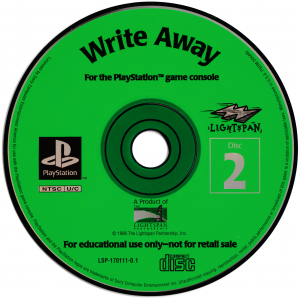
\includegraphics[width=\textwidth/2]{./Games/WriteAway/Images/WriteAway2CD.png}
    \caption{Write Away 2 CD}
\end{figure}

The second of the ten Write Away games published and released by The Lightspan Partnership for the PlayStation 1.

Write Away 2 features ten video programs, including an introduction video, eight story videos, and a conclusion video:

\begin{itemize}
    \item Write Away Episode Two Introduction
    \item The Space Adventure by Emily Barkelew \& Alexandra Gibney
    \item I Hate the Fall by Stephanie Sentel
    \item The Monster That Jean Scared by Jean Lowrey
    \item How to Brush Your Teeth by John Knight
    \item Hair by Brittany Cantrell
    \item Frasier's Big Weekend by Clark Munson
    \item Chester the Crocodile by Ms. Brozda's Class
    \item Brattylocks by Meredith Sutton
    \item Write Away Conclusion
\end{itemize}

\clearpage
\newpage

\section{Transcriptions}

\subsection{The Space Adventure by Emily Barkelew \& Alexandra Gibney}

TODD:
I'd love to go to the library to read books about science fiction and space.

ELISE:
Ssh.

TODD:
I hope someday I'll get to travel in a rocket ship and walk on the moon.

ELISE:
Ssh.

TODD:
And maybe if I ever get to space, I'll have some interesting companions just like the ones written by fourth-grader Emily Barkelew and kindergartner Alexandra Gibney.
They go to the Alps Road School in Athens, Georgia.
Watch with me their exciting story, "The Space Adventure".

DEBORAH (VOICE OVER):
Once there was a famous astronaut named Skip.
He was going to the moon.
What he didn't know was that three of his biggest fans had followed him to the spaceship.
There was Brett the lion.

BRETT THE LION:
I can't wait to get his autograph.
Rawh!

DEBORAH (VOICE OVER):
And Maddie the tiger.

MADDIE THE TIGER:
I'm gonna take his picture.
Rawr!

DEBORAH (VOICE OVER):
And a cheetah named Emily.

EMILY THE CHEETAH:
I just want to touch him.
Prrr!

DEBORAH (VOICE OVER):
All of a sudden, the animals heard Skip say...

SKIP:
Mission control, five, four, three, two, one, blast off!

DEBORAH (VOICE OVER):
Finally, the spaceship landed.

SKIP:
Mission control, I'm now going to take a walk on the moon.

EMILY THE CHEETAH:
Pst.
He's going for a walk, let's follow him.

BRETT THE LION:
This is so exciting!

MADDIE THE TIGER:
Ssh.

DEBORAH (VOICE OVER):
The animals followed Skip until he heard footsteps behind him.

SKIP:
I hear something behind me, but that's no problem though because I'm astronaut Skip.
Aah! Aah!

DEBORAH (VOICE OVER):
The astronaut ran back to the spaceship and blasted off, leaving the three animals behind.

SKIP:
Mission control, it was awful.
There's creatures attacking me from all sides.
I think I'll write a book about it and make lots of money.

DEBORAH (VOICE OVER):
As for the three animals...

BRETT THE LION:
I didn't get his autograph.

MADDIE THE TIGER:
I forgot to turn the flash on.

EMILY THE CHEETAH:
Let's not worry about that now, we're stranded.

DEBORAH (VOICE OVER):
Suddenly, they met an alien, a friendly alien, who adopted them, and they spent the rest of their lives on the moon.

EIMLY THE CHEETAH, MADDIE THE TIGER, BRETT THE LION:
[We're ever so humble, there's no] place like the moon.

DEBORAH (VOICE OVER):
And they were always happy.

\subsection{I Hate the Fall by Stephanie Sentel}

PAUL:
Potato, Tomato, Clock, Block.

ELISE:
What are you doing?

PAUL:
Oh, I'm writing a poem.

ELISE:
A poem?

PAUL:
Yeah, all you have to do is rhyme, right?

ELISE:
Well, rhyming is part of it, but a poem can also be a story about something you like or maybe about something you don't like.
That's what fifth-grader Stephanie Sentel from Magawa Elementary did. It's entitled 'I Hate Fall.'

WOMAN 1:
I hate falling when I'm running a race,
Because when I fall, I fall on my face.
I hate it when a brick falls.
Oh no!
Especially when it lands on my toe.

MAN 1:
Sorry.

WOMAN 1:
Then I mumble and grumble and say words I shouldn't.

WOMAN 2 AND MAN 1:
Uh uh uh.

WOMAN 1:
Cus it isn't okay.
I hate it when leaves fall to the ground.
I'm just glad they don't weigh a pound.
I hate fall.
The End.

\subsection{The Monster That Jean Scared by Jean Lowrey}

NARRATOR:
And now, welcome to another spine-tingling tale from the script.

PAUL:
Welcome, and I'm glad you're here for another scary story.
One of the scariest things is a monster.
What's even scarier is when you put yourself in a story with a monster, and that's exactly what Jean Lowrey did, a second-grader from Midland Elementary, in her deliciously scary tale entitled "The Monster That Jene Scared."
Sounds exciting.

PAUL (VOICE OVER):
One day, three friends, Amanda.

AMANDA:
Like, hi.

PAUL (VOICE OVER):
Jean.

JEAN:
Hi.

PAUL (VOICE OVER):
And Jenny.

JENNY:
Hi.

PAUL (VOICE OVER):
Were walking down the street, when all of a sudden a monster popped up from behind a rock.

MONSTER:
Eeny meeny miny moe, I'll take you, and away we'll go.

PAUL (VOICE OVER):
The monster kidnapped Amanda.

JEAN:
What do you think, Amanda?

JEAN AND JENNY:
Amanda?

PAUL (VOICE OVER):
They saw that Amanda was gone.
They looked everywhere for her.

JEAN:
She's gone.

JENNY:
I think Amanda's been kidnapped."

JEAN:
And look, there are two sets of footprints.
One going like this, and the other one like this.

JENNY:
Cool. How'd you do that?

JEAN:
Well, you put one hand here and you...
Oh, we don't have time for this.
Look, these are leading right up to that spooky castle.

JENNY:
I have an idea.
Let's find Amanda and rescue her.

JEAN:
Okay.

JEAN AND JENNY:
Huh.

MONSTER:
Here's me as a baby.
And here's me at prom... Alone.
Oh, the tea is ready.
I'll be back.

JEAN:
There she is.

JENNY:
Let's rescue her and go.

PAUL (VOICE OVER):
But just as they were about to rescue her...

MONSTER:
So, you thought you'd try and save your little friend.
Well, now I've got the three of you.

JEAN:
My - Aah!

JENNY:
Oh yeah?
Well, you don't scare me.

MONSTER:
[Really], oink.

JENNY:
Why don't you just go away?

MONSTER:
Hhh...

JENNY:
And while you're at it, take a bath.
Do something about that breath, clean up this place.
It's disgusting.
You're disgusting.
Everything's disgusting.

PAUL (VOICE OVER):
Gene was so brave that she scared the monster off.

AMANDA:
Like you saved us all.
And you know what?

JEAN AND JENNY:
What?

AMANDA:
Like, It's my birthday.

JEAN AND JENNY:
Aah!

PAUL (VOICE OVER):
The three girls went home and had cake and ice cream and partied away.

AMANDA, JEAN, JENNY:
Like, for sure.

PAUL:
Ooh, a cake and ice cream party.
Oh, like, for sure.
Now that sounds scary.
And I'm looking forward to more tales of terror and suspense from all you authors out there to be presented on our next 'Tales from the Script'.
Ta-ta for now.

\subsection{How to Brush Your Teeth by John Knight}

ELISE:
You add one cup of sugar and mix thoroughly.

SABRINA:
Hey Elise, you know you're reading a very important form of writing.

ELISE:
What are you talking about, Sabrina? All I'm doing is reading the instructions on how to make cupcakes.

SABRINA:
Well, if a writer a long time ago had not taken the time to write down how to make cupcakes, then you wouldn't know how, and we wouldn't have dessert.
In fact, we might not know how to do a lot of things like building a plane or working a computer.
That's what second-grader John Knight from Town Point Elementary did in his story, 'How to Brush Your Teeth.'

MAN 1:
First, you get your toothbrush.

MAN 2, WOMAN 1, WOMAN 2, WOMAN 3:
First, you get your toothbrush.

MAN 1:
Then, you get your toothpaste.

MAN 2, WOMAN 1, WOMAN 2, WOMAN 3:
Then, you get your toothpaste.

MAN 1:
Then you wet your toothbrush.

MAN 2, WOMAN 1, WOMAN 2, WOMAN 3:
Then you wet your toothbrush.

MAN 1:
Then you brush your teeth.

MAN 2, WOMAN 1, WOMAN 2, WOMAN 3:
Then you brush your teeth.
Mmm hmm mmm hmm mmm.

MAN 1:
Then you get a cup.

MAN 2, WOMAN 1, WOMAN 2, WOMAN 3:
Then you get a cup.

MAN 1:
Then you get some water.

MAN 2, WOMAN 1, WOMAN 2, WOMAN 3:
Then you get some water.

MAN 1:
Then you spit it out.

MAN 2, WOMAN 1, WOMAN 2, WOMAN 3:
Mmm hmm mmm hmm mmm.

MAN 1:
Then you wipe your mouth.

MAN 2, WOMAN 1, WOMAN 2, WOMAN 3:
Then you wipe your mouth.

MAN 1:
And then\dots you're\dots done.
How to brush your teeth.
The end.

\subsection{Hair by Brittany Cantrell}

DEBORAH:
An exciting thing about writing is that you're totally in charge.
Now, there are many ways in which you can start a story, and you can decide which way to choose.
You might want to start with a narrator telling the story:
Once upon a time, there was a girl named Sally.
Or you can do like Brittany Cantrell from Independence Elementary School did, where she took her main character, Sally, and let her tell the story of hair.

SALLY:
Hi, my name's Sally, and I really hate my hair.
So I decided to ask my family what to do.
Mom, what should I do with my hair?

MOM:
Cut it short.

SALLY:
Dad, what should I do with my hair?

DAD:
Grow bangs.

SALLY:
Sis, what should I do with my hair?

SISTER:
Get a perm.

SALLY:
Hey, brother, what should I do with my hair?

BROTHER:
Just keep it the same.

SALLY:
I couldn't decide, so I decided to ask my neighbors, the Cool's.
They have really cool taste.
Well, here goes nothing.
Mrs. Cool, what should I do with my hair?

MRS. COOL:
Well, honey, I think you should get some pigtails.

SALLY:
I think I'll ask Mr. Cool.
Mr. Cool, what should I do with my hair?

MR. COOL:
Red hair, now that's the trick.

MRS. COOL:
Curl it, call it big like this.

MR. COOL:
No, what every young girl needs is a topsy tail.

MRS. COOL:
A bun.

MR. COOL:
A topsy tail.

MRS. COOL:
A bun

MR. COOL:
A topsy tail.

SALLY:
So, I went home and sat in my tree for a long time.
I guess my brother was right.
I'll keep my hair just the way it is.
But now, what am I gonna wear?

\subsection{Frasier's Big Weekend by Clark Munson}

ELISE:
What are you two laughing about?

TODD:
This Danny Duck is so funny.

SABRINA:
The way he always fools Pete Bunny really quacks me up.

ELISE:
Oh, so you guys like stories with personification.

SABRINA, TODD:
Persona-what?

ELISE:
Personification.
See, that's when an author gives human characteristics to things.
Like animals.
That's how Danny Duck can talk and sing.
And you should see how our next author uses personification.
Clark Munson, a fifth-grader from Villa Park Elementary, gives Frasier the dog a very funny personality in 'Frasier's Big Weekend'.

FRASIER:
Hello, my name is Frasier, and I'm -.

OWNER:
Leaving now Frasier.
Be a good boy, and take care of the house.

FRASIER:
And that's my owner, and he's finally going on vacation for the weekend, and that means party party party.
So, I just do my good dog thing.
I just sit here and I wag my tail as I watch him leave.
As soon as he gets around the corner, I'm out of my doghouse on the way to the park.

I like going to the park, and I love laying in the sand and wiggling.
Oh, that's good.
Oh yeah, oh yeah, that's good.

Hey, hey, there's Mrs. Salem.
She makes the best sandwiches.
She puts plenty of turkey on them.
They are yummy to my tummy, and she always has a spare one for me.

MRS. SALEM:
Oh, Frasier, what a nice dog.

FRASIER:
Oh look, it's my good buddies Lassie and Baby Joe.
They're the best.
We like to run, play tag, you're it.
Hey look, our big thrill is to munch down on somebody else's goodies.
A big juicy bone, wow.

Well, see you later guys.
I gotta go see my sweetheart Lady.
What a babe.
We rub noses and say hello.
Hi.

LADY DOG:
Hello Frasier.

FRASIER:
What do you want to do?

LADY DOG:
Let's go over zere and watch ze ducks in ze moonlight, and then we can go have some ice cream.

FRASIER:
Sure.
Oh look, somebody left a picnic basket and a blanket so that we can have a midnight dinner.

LADY DOG:
Are you going to finish that?

FRASIER:
No.
Ain't she something.
Ah.
Well, too bad we had to end it early because my owner was coming home early in the morning.
So, I kissed my sweetheart good night.
See you.

I quickly got into my doghouse as my owner pulled in the driveway, and I just sat there and did my good dog thing, wagging my tail, and I greeted him.

OWNER:
Oh I missed you so much Frasier.

FRASIER:
What a weekend.
I wish it would never end.
I wonder when my owner's gonna go away again.

OWNER:
Next time I go on vacation, I'm going to take you with me.

FRASIER:
Oh no.

\subsection{Chester the Crocodile by Ms. Brozda's Class}

PAUL:
I always like it when a story can teach me something, but what's even better is when that same story can entertain me and make me laugh.
And that's what a group of writers did from Ms. Bros' second-grade class at Kings Elementary in their story entitled 'Chester the Crocodile.'

ELISE (VOICE OVER):
Once upon a time, there lived a crocodile named Chester who loved to eat candy.

CHESTER:
I love candy.
I can't get enough of it.
I ate it for breakfast, mmm\dots
Jelly beans.
Oh, and for lunch, licorice.
We mustn't forget dinner, chocolate.
Oh, and dessert.

ELISE (VOICE OVER):
Suddenly, he got a terrible toothache.

CHESTER:
Oh no.
Mom, every one of my teeth is killing me.
Every one of them aches.

MOM:
I think you've been eating too much candy.
I think it's now time for a trip to the dentist.

CHESTER:
Oh no, not the dentist.

ELISE (VOICE OVER):
Chester and his mom went to the dentist's office.

RECEPTIONIST:
Welcome to Dr. Bucky Bunny's.
How may I help you?

MOM:
Oh, my son has a terrible toothache.
I think he's eating too much candy.

RECEPTIONIST:
Follow me.

ELISE (VOICE OVER):
Chester climbed into the dentist chair and began to cry.

CHESTER:
I ate too much candy.

DENTIST:
Oh, don't cry, Chester.
Let me take a look.
Oh, this doesn't look good.
You're gonna have to have all your teeth taken out because you ate too much candy.

ELISE (VOICE OVER):
So, the dentist pulled all of Chester's teeth out.

DENTIST:
Now, remember, Chester, when your teeth grow back, don't eat so much candy.
Eat more fruit, and always brush your teeth.

CHESTER:
Don't worry, I'll eat right from now on.

ELISE (VOICE OVER):
And from that day on, Chester never ate candy again, and all of his teeth did grow back.
Now, the moral of this story is\dots

CHESTER:
Don't eat too much candy.

DENTIST:
And always brush your teeth.
Next.

\subsection{Brattylocks by Meredith Sutton}

SABRINA:
And they lived happily ever after.
Hmm, I wonder.

TODD:
Wonder what, Sabrina?

SABRINA:
I wonder what really happens when these fairy tales end.
I'd like to see a well-known story like 'Goldilocks and the Three Bears' retold from a different point of view.

TODD:
Well, you're in luck.
That's what we'll see in 'Bratty Locks', the story written by sixth-grader Meredith Sutton from Lowell Elementary.

TODD (VOICE OVER):
Once upon a time, there lived three bears.
Yes, the papa bear, the mama bear, and of course, the baby bear.

MAMA BEAR:
Oh, this porridge is too hot.
Why don't we go for a walk while it cools off?

TODD (VOICE OVER):
So, they went for a walk, and no sooner had they left than a bratty little girl named Bratty Locks came upon the cottage.

BRATTY LOCKS:
Huh, everyone thinks I'm my twin sister Goldilocks, but I ain't.
I'm Bratty Locks, and I'm here to show those bears what I'm made of.

TODD (VOICE OVER):
Now, Goldilocks would have knocked on the door, but\dots

BRATTY LOCKS:
I ain't her. Haiya!

TODD (VOICE OVER):
So, she kicked the door open and went inside.

BRATTY LOCKS:
Hmm\dots
Look, porridge, and me without a meal for at least an hour.
Oh, this one's too hot.
Oh, this one's too cold.
This one's just right.
Pff, my sister would eat this chunk, but I'm gonna put it down the garbage disposal.

TODD (VOICE OVER):
And that's what she did.

BRATTY LOCKS:
Well, that's done.
Now to rearrange the living room furniture.
This one's too big.
I'll never get it out the window.
This one's too soft; it won't even break.
Ah, this one's just right.

TODD (VOICE OVER):
Bratty Locks picked up the baby bear's chair and threw it out the window, and it broke.

BRATTY LOCKS:
I wonder what's over there.
Let's go see.

TODD (VOICE OVER):
Bratty Locks ran to the three beds.
She jumped on the big one, messed the middle one up, and threw the bedspread of the little one on the floor.

BRATTY LOCKS:
Now to wait for those silly little bears to come home.

TODD (VOICE OVER):
The three unsuspecting bears came home from their walk.

PAPA BEAR:
Well, Goldie, what are you doing here?

BRATTY LOCKS:
I'm not Goldilocks; I'm Bratty Locks, and I'm here to pay you back for mistaking me for my goody-two-shoes sister.

BABY BEAR:
Look, she dumped all her food in the sink, and she threw my chair out the window!

BRATTY LOCKS:
And I messed up your beds too.
Ha ha ha.

PAPA BEAR:
Thank you, Bratty Locks. We were all done with our porridge.

MAMA BEAR:
Oh, and we're getting a new set of chairs and table today.

BABY BEAR:
And today's the day we change the sheets.

PAPA BEAR, MAMA BEAR, BABY BEAR:
Thank you Bratty Locks.

TODD (VOICE OVER):
Bratty Locks was amazed and began to cry.

BRATTY LOCKS:
It's not fair! It's not fair!

BABY BEAR:
Works every time.

\subsection{Write Away Conclusion}

DEBORAH:
We hope you enjoyed our show today.
Your stories are finished and all put away.

TODD:
but we'll come again another day.

SABRINA
The stories you've seen through music and mime\dots

ELISE:
Can be written by you if you just take the time.

PAUL:
So, pick up your pencil and paper. You'll see\dots

TOGETHER:
The adventures of magic that writing sets free.
So, write away.

\section{Credits}